\documentclass[12pt]{kiarticle} % You can learn about my document class "kiarticle" and install it to your device by following the link: https://github.com/Kiarendil/toolkitex
\graphicspath{{pictures/}}
\DeclareGraphicsExtensions{.pdf,.png,.jpg,.eps}
%%%
\pagestyle{fancy}
\fancyhf{}
%\renewcommand{\headrulewidth}{ 0.1mm }
\renewcommand{\footrulewidth}{ .0em }
\fancyfoot[C]{\texttt{\textemdash~\thepage~\textemdash}}
\fancyhead[L]{Лабораторная работа № 4.2.1 \hfil}
\fancyhead[R]{\hfil Иванов Кирилл, 625 группа }
\usepackage{multirow} % Слияние строк в таблице
\newcommand
{\un}[1]
{\ensuremath{\text{#1}}}
\newcommand{\eds}{\ensuremath{ \mathscr{E}}}
\usepackage{tikz}
%%% Работа с таблицами
\usepackage{array,tabularx,tabulary,booktabs} % Дополнительная работа с таблицами
\usepackage{longtable}  % Длинные таблицы
\usepackage{multirow} % Слияние строк в таблице

\begin{document}
	
	\begin{titlepage}
	\begin{center}
		\large 	Московский физико-технический институт \\
		(государственный университет) \\
		Факультет общей и прикладной физики \\
		\vspace{0.2cm}
		
		\vspace{4.5cm}
		Лабораторная работа № 4.2.1 \\ \vspace{0.2cm}
		\large (Общая физика: оптика) \\ \vspace{0.2cm}
		\LARGE \textbf{Кольца Ньютона}
	\end{center}
	\vspace{2.3cm} \large
	
	\begin{center}
		Работу выполнил: \\
		Иванов Кирилл,
		625 группа
		\vspace{10mm}		
		
	\end{center}
	
	\begin{center} \vspace{60mm}
		г. Долгопрудный \\
		2018 год
	\end{center}
\end{titlepage}
	
	\paragraph*{Цель работы:} познакомиться с явлением интерференции в тонких плёнках (полосы равной толщины) на примере колец Ньютона и с методикой интерференционных измерений кривизны стеклянной поверхности.
	
	\paragraph*{Оборудование:} измерительный микроскоп с опак-иллюминатором, плоско-выпуклая линза; пластинка из чёрного стекла, ртутная лампа типа ДРШ, щель, линзы, призма прямого зрения, объектная шкала.
	
	\section{Теоретическое введение}
	
	\begin{wrapfigure}{l}{0.35\linewidth} 
		\includegraphics[width=\linewidth]{ring}
		\caption{Экспериментальная установка}
		\label{ring}
	\end{wrapfigure}

	Этот классический опыт используется для определения радиуса кривизны сферических поверхностей линз. В этом опыте наблюдается интерференция волн, отражённых от границ тонкой воздушной прослойки, образованной сферической поверхностью линзы и плоской стеклянной пластиной. При нормальном падении света (рис. \ref{ring}) интерференционные полосы локализованы на сферической поверхности и являются полосами равной толщины.
	
	Геометрическая разность хода между интерферирующими лучами равна удвоенной толщине воздушного зазора $ 2d $ в данном месте. Для точки на сферической поверхности, находящейся на расстоянии $ r $ от оси системы, имеем $ r^2 = R^2 - (R - d)^2 = 2Rd - d^2 $, где $ R $ --- радиус кривизны сферической поверхности (рис. \ref{ring}).
	
	При $ R \gg d $ получим$  d = r^2/2R $. С учётом изменения фазы на $ \pi $ при отражении волны от оптически более плотной среды (на границе воздух-стекло) получим \textbf{оптическую разность хода интерферирующих лучей}:
	
	\begin{equation}\label{r_m}
	\Delta = \dfrac{\lambda}{2} + 2d = \dfrac{r^2}{2R} + \dfrac{\lambda}{2}
	\end{equation}
	
	Из условия интерференционного минимума $ \Delta = \dfrac{(2m +1)\lambda}{2}, \; m =0, 1, 2.. $ получим радиусы темных колец $ r_m $, а из аналогичного условия максимума $ \Delta = m \lambda $ радиусы светлых $ r_m' $ :
	
	\begin{equation}\label{r_m'}
	r_m = \sqrt{m \lambda R}, \qquad 	r_m' = \sqrt{\dfrac{(2m-1)m \lambda R}{2}}
	\end{equation}
	
	\section{Экспериментальная установка}

Схема экспериментальной установки приведена на рис. \ref{lab}. Опыт выполняется с помощью измерительного микроскопа.
На столик микроскопа помещается держатель с полированной пластинкой из
чёрного стекла. На пластинке лежит исследуемая линза.

	\begin{wrapfigure}{r}{0.5\linewidth} 
	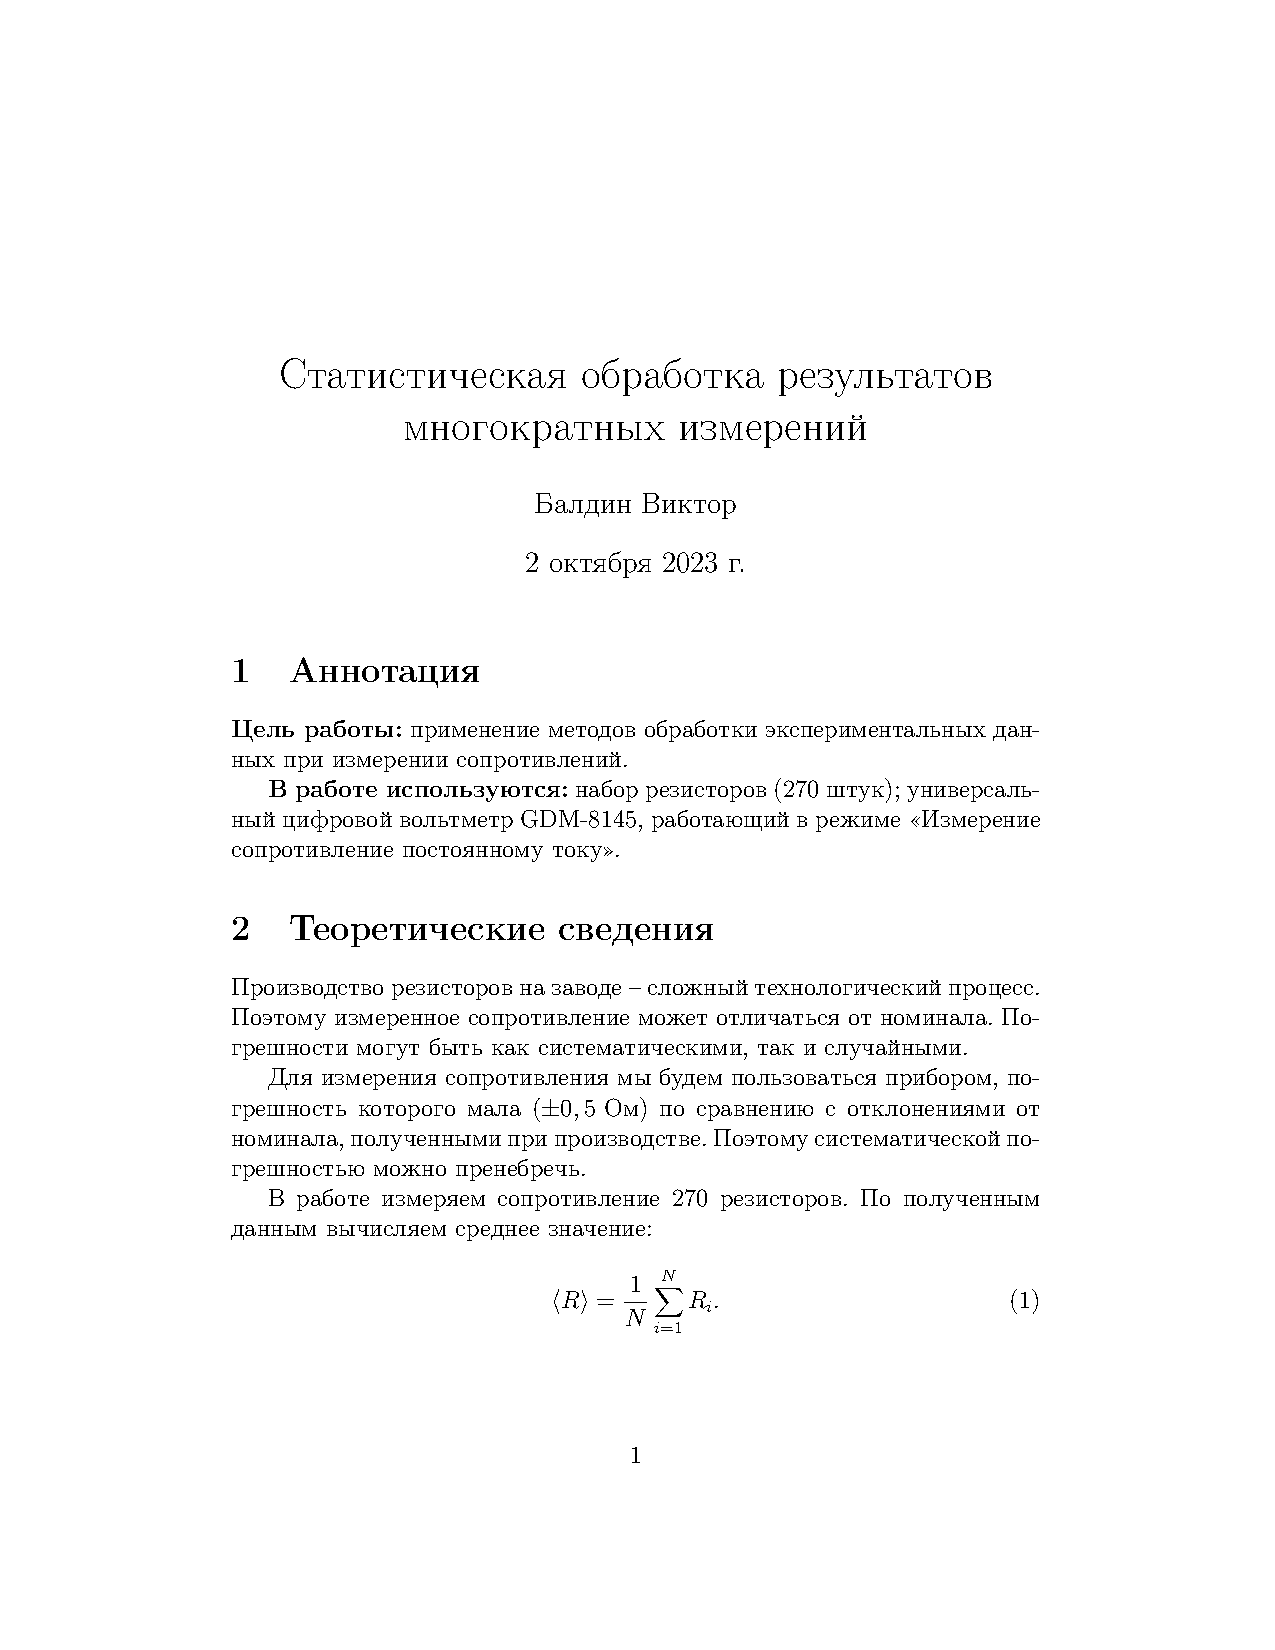
\includegraphics[width=\linewidth]{lab}
	\caption{Экспериментальная установка}
	\label{lab}
\end{wrapfigure}

	Источником света служит ртутная лампа, находящаяся в защитном кожухе. Для получения монохроматического света применяется призменный монохроматор, состоящий из конденсора $ К $, коллиматора (щель $ S $ и объектив $ О $) и призмы прямого зрения $ П $. Эти устройства с помощью рейтеров располагаются на оптической скамье. Свет от монохроматора попадает на расположенный между объективом и окуляром микроскопа опак-иллюминатор (ОИ)  специальное устройство, служащее для освещения объекта при работе в отражённом свете. Внутри опак-иллюминатора находится полупрозрачная стеклянная пластинка P, наклоненная под углом $ 45^\circ $ к оптической оси микроскопа. Свет частично отражается от этой пластинки, проходит через объектив микроскопа и попадает на исследуемый объект. Пластинка может поворачиваться вокруг горизонтальной оси $ X $, опак-иллюминатор вокруг вертикальной оси.

	Столик микроскопа может перемещаться в двух взаимно перпендикулярных направлениях помощью винтов препаратоводителя. Отсчетный крест окулярной шкалы перемещается перпендикулярно оптической оси с помощью микрометрического винта $ М $.
	
	Оптическая схема монохроматора позволяет получить в плоскости входного окна опак-иллюминатора достаточно хорошо разделённые линии спектра ртутной лампы. Изображение щели $ S $ фокусируется на поверхность линзы объективом микроскопа, т.е. точка источника и точка наблюдения спектра совпадают.Интерференционная картина не зависит от показателя преломления линзы и определяется величиной зазора между линзой и пластинкой (кольца равной толщины).

	Сначала микроскоп настраивается на кольца Ньютона в белом свете (свете ртутной лампы), затем при помощи монохроматора выделить из спектра яркую зелёную линию и провести измерения диаметров колец в монохроматическом свете. 
	
		\begin{table}[h!]
		\caption{Измерение диаметров колец Ньютона}
		\begin{center}
			\begin{tabular}{|c|c|c|c|c|c|c|}
				\hline
				m & \multicolumn{3}{|c|}{Темные кольца} & \multicolumn{3}{|c|}{Светлые кольца} \\
				\cline{2-7}
				& $ l_1 $& $ l_2 $ & $ r_m^2 $ &$ l_1 $& $ l_2 $ & $ (r_m')^2 $ \\
				\hline
				0 & 4.71 & 3.72 & 0.25 & 4.15 & 4.15 & 0 \\
				1 & 5 & 3.24 & 0.77 & 4.78 & 3.43 & 0.46 \\
				2 & 5.45 & 2.92 & 1.6 & 5.16 & 3.08 & 1.08 \\
				3 & 5.59 & 2.65 & 2.16 & 5.44 & 2.79 & 1.76 \\
				4 & 5.83 & 2.42 & 2.91 & 5.7 & 2.54 & 2.5 \\
				5 & 6.02 & 2.23 & 3.59 & 5.91 & 2.32 & 3.22 \\
				6 & 6.17 & 2.06 & 4.22 & 6.09 & 2.11 & 3.96 \\
				7 & 6.47 & 1.89 & 5.24 & 6.25 & 1.97 & 4.58 \\
				\hline
			\end{tabular}
		\end{center}
		\label{table}
	\end{table}
	
	
	\section{Ход работы}
	
	После настройки микроскопа проведем измерения диаметров колец Ньютона. Измерения будем проводить в безразмерных единицах окулярной шкалы, переведённых затем в реальную величину с помощью калиброванной объектной шкалы. 
	
	
	Оценим систематическую погрешность измерения величин на окуляре как $ \sigma_l = 0,02 $ (из-за цены деления).
	
	C помощью призмы разобьем свет ртутной лампы на зеленый ($ \lambda_з = 546 $ нм) и желтый ($ \lambda_ж = 578  $ нм).
	
	Будем последовательно измерять расстояния $ l_1 $ от верхнего края 6-ого "<набора"> колец до нуля до центра, затем аналогично будем измерять расстояния $ l_2 $ от нижнего края до нуля. Результаты занесем в таблицу. 
	
		\begin{figure}[h!]
		\label{graf}
		\includegraphics[scale=0.47]{graf.pdf}
		\caption{График зависимости $ r_m^2$ и $ (r_m')^2 $ от номера $ m $}
	\end{figure}
	
	Построим график зависимости радиусов колец от их номера. 

	\begin{table}[h!]
		\centering
		\caption{Расчет апроксимированной прямой $ y = ax +b $ для темных колец}
		\begin{tabular}{l|ll}
				\text{} & \text{Estimate} & Standart Error  \\
				\hline
				$ b $ & 0.13 & 0.08  \\
				$ a $ & 0.70 & 0.01  \\
			\end{tabular}
	\end{table}

	\begin{table}[h!]
		\centering
		\caption{Расчет апроксимированной прямой $ y = ax +b $ для светлых колец}
		\begin{tabular}{l|ll}
			\text{} & \text{Estimate} & Standart Error  \\
			\hline
			$ b $ & -0.17 & 0.06 \\
	$ 	a $ & 0.67 & 0.01
		\end{tabular}
	\end{table}

	Теперь определим калибровку окулярной шкалы. Она равна $ k = 0,1 $ мм.

	При биениях мы наблюдали следующее количество полос между центрами четких систем $ \Delta m =  12 $. Вычислим отсюда разность длин волн желтого и зеленого света ртутной лампы $ \Delta \lambda = \lambda_ж - \lambda_з $:
	
	\begin{equation}\label{}
	(\Delta m + 1)\lambda_з = \Delta m \lambda_ж \te \Delta \lambda = \dfrac{\lambda_з}{\Delta m} \approx 45 \; нм
	\end{equation}

	Определим радиус кольца. Так как $ \dfrac{r^2_m}{m} = k^2 \x a_т$, отсюда

	\begin{equation}\label{}
	R = \dfrac{r^2_m}{m \lambda} = (1,28 \pm 0,02) \; см
	\end{equation}
	
	\section{Вывод}
	
	Таким образом, мы получили, что их экспериментального периода биений разница длин волн  желтого и зеленого света ртутной лампы примерно равна \fbox{$  \Delta \lambda = 45 \; нм $}, в то время как табличный результат --- 33 нм. Это может быть объяснено большой неточностью определения числа $ \Delta m $.
	
	Также мы построили графики зависимости радиусов колец Ньютона от их номеров. Полученный результат позволил нам рассчитать радиус линзы ---  \fbox{$ R = (1,28 \pm 0,02) \; см $}.
	
	
	
	
	
\end{document}
